\setcounter{section}{29}
\section{Đa giác đều}

% Nguồn SGK: Bài 30, trang 84--89 theo direct image URL trong issue #22.
% Nguồn SBT: SBT TOÁN 9 TẬP 2.pdf trong Project Sources, PDF trang 59--60,
% SHA-256 5ff01fd213d1adc75f9c54b4408d6a9642a4d8038e685040efef3311a196196c.

\begin{lesson}
    \subsection{Kiến thức trọng tâm}

    \begin{center}
        \begin{tblr}{
            width=\linewidth,
            colspec={X[l] X[l]},
            cells={valign=t},
            row{1}={font=\bfseries, halign=c}
        }
            Khái niệm, thuật ngữ & Kiến thức, kĩ năng \\
            \textbullet\ Đa giác, đa giác đều\par
            \textbullet\ Đỉnh, cạnh, góc của đa giác\par
            \textbullet\ Phép quay
            &
            \textbullet\ Nhận dạng đa giác đều. Nhận biết những hình phẳng đều trong tự nhiên, nghệ thuật, kiến trúc, công nghệ chế tạo,\ldots\par
            \textbullet\ Nhận biết vẻ đẹp của thế giới tự nhiên biểu hiện qua tính đều.\par
            \textbullet\ Nhận biết phép quay. Mô tả được các phép quay giữ nguyên hình đa giác đều.
        \end{tblr}
    \end{center}

    Chúng ta đã biết tam giác đều được tạo bởi ba cạnh bằng nhau, hình vuông được tạo bởi bốn cạnh bằng nhau. Hơn nữa, các góc trong mỗi hình đó bằng nhau. Trong bài này các em sẽ được học về những hình tương tự như vậy nhưng số cạnh có thể nhiều hơn, chúng được gọi chung là các đa giác đều.

    \textbf{1. ĐA GIÁC ĐỀU}

    \textbf{Đa giác}

    Những hình như Hình 9.38 được gọi chung là các đa giác.

    % TODO(HINH-NGUON): bo sung asset/crop dung Hinh 9.38 tu SGK trang 84; khong redraw xap xi bang TikZ.

    Đa giác $ABCDE$ (H.9.38a) là những hình gồm năm đoạn thẳng $AB$, $BC$, $CD$, $DE$, $EA$, trong đó bất kì hai đoạn thẳng nào có một điểm chung cũng không cùng nằm trên một đường thẳng. Đa giác $ABCDE$ có năm đỉnh là các điểm $A$, $B$, $C$, $D$, $E$, năm cạnh là các đoạn thẳng $AB$, $BC$, $CD$, $DE$, $EA$ và năm góc là các góc $EAB$, $ABC$, $BCD$, $CDE$, $DEA$.

    Nếu với một cạnh bất kì, các đỉnh không thuộc cạnh đó đều nằm về một phía đối với đường thẳng chứa cạnh đó thì đa giác được gọi là đa giác lồi. Các đa giác trong Hình 9.38 a, b, d là các đa giác lồi. Đa giác trong Hình 9.38c không phải đa giác lồi.

    \textbf{Đa giác đều}

    \textbf{HĐ1} Ta đã biết các tam giác đều và hình vuông có các đỉnh nằm trên một đường tròn. Ta dựng một đa giác lồi 5 cạnh có các đỉnh nằm trên một đường tròn như sau:
    \begin{itemize}
        \item Vẽ đường tròn tâm $O$ bán kính $R$.
        \item Lần lượt lấy các điểm $A$, $B$, $C$, $D$, $E$ trên đường tròn theo thứ tự ngược chiều kim đồng hồ (hoặc theo chiều kim đồng hồ) sao cho:
        \[
            \widehat{AOB}=\widehat{BOC}=\widehat{COD}=\widehat{DOE}=\widehat{EOA}
            =\dfrac{360^\circ}{5}=72^\circ.
        \]
    \end{itemize}
    Em hãy giải thích vì sao các cạnh và các góc của đa giác $ABCDE$ bằng nhau (H.9.39).

    \begin{center}
        \begin{tikzpicture}[scale=0.9]
            \coordinate (O) at (0,0);
            \foreach \name/\ang in {A/90,B/18,C/-54,D/-126,E/162}{
                \coordinate (\name) at (\ang:2);
            }
            \draw (O) circle (2);
            \draw (A)--(B)--(C)--(D)--(E)--cycle;
            \foreach \name in {A,B,C,D,E}{\draw (O)--(\name);}
            \fill (O) circle (1.2pt);
            \node[below=1pt of O] {$O$};
            \node[above=1pt of A] {$A$};
            \node[right=1pt of B] {$B$};
            \node[below right=1pt of C] {$C$};
            \node[below left=1pt of D] {$D$};
            \node[left=1pt of E] {$E$};
        \end{tikzpicture}

        \textit{Hình 9.39}
    \end{center}

    \answerline
    \answerline

    Đa giác $ABCDE$ như Hình 9.39 được gọi là một đa giác đều. Tổng quát, ta có định nghĩa:

    \begin{keyconcept}
        Đa giác đều là một đa giác lồi có các cạnh bằng nhau và các góc bằng nhau.
    \end{keyconcept}

    Người ta chứng minh được rằng các đỉnh của mỗi đa giác đều luôn cùng nằm trên một đường tròn, được gọi là đường tròn ngoại tiếp đa giác, tâm đường tròn được gọi là tâm của đa giác và đa giác được gọi là nội tiếp đường tròn đó.

    \textbf{Câu hỏi} Nếu một lục giác đều (đa giác đều 6 cạnh) nội tiếp đường tròn bán kính 2 cm (H.9.40) thì độ dài các cạnh của lục giác đều bằng bao nhiêu centimét? Số đo các góc của lục giác đều bằng bao nhiêu độ?

    \begin{center}
        \begin{tikzpicture}[scale=0.8]
            \coordinate (O) at (0,0);
            \foreach \name/\ang in {A/0,B/60,C/120,D/180,E/240,F/300}{
                \coordinate (\name) at (\ang:2);
            }
            \draw (O) circle (2);
            \draw (A)--(B)--(C)--(D)--(E)--(F)--cycle;
            \fill (O) circle (1.2pt);
            \node[below=1pt of O] {$O$};
        \end{tikzpicture}

        \textit{Hình 9.40}
    \end{center}

    \answerline
    \answerline

    \textbf{Luyện tập 1}

    Cho $M$, $N$, $P$, $Q$, $K$ lần lượt là trung điểm của các cạnh $AB$, $BC$, $CD$, $DE$ và $EA$ của ngũ giác đều $ABCDE$ (H.9.44). Hỏi $MNPQK$ có phải là ngũ giác đều hay không?

    \begin{center}
        \begin{tikzpicture}[scale=0.9]
            \foreach \name/\ang in {A/90,B/18,C/-54,D/-126,E/162}{
                \coordinate (\name) at (\ang:2.2);
            }
            \coordinate (M) at ($(A)!0.5!(B)$);
            \coordinate (N) at ($(B)!0.5!(C)$);
            \coordinate (P) at ($(C)!0.5!(D)$);
            \coordinate (Q) at ($(D)!0.5!(E)$);
            \coordinate (K) at ($(E)!0.5!(A)$);
            \draw (A)--(B)--(C)--(D)--(E)--cycle;
            \draw (M)--(N)--(P)--(Q)--(K)--cycle;
            \node[above=1pt of A] {$A$};
            \node[right=1pt of B] {$B$};
            \node[below right=1pt of C] {$C$};
            \node[below left=1pt of D] {$D$};
            \node[left=1pt of E] {$E$};
            \node[above right=1pt of M] {$M$};
            \node[right=1pt of N] {$N$};
            \node[below=1pt of P] {$P$};
            \node[left=1pt of Q] {$Q$};
            \node[above left=1pt of K] {$K$};
        \end{tikzpicture}

        \textit{Hình 9.44}
    \end{center}

    \answerline
    \answerline

    \textbf{Thử thách nhỏ 1} Cho một bát giác đều (đa giác đều 8 cạnh) nội tiếp một đường tròn tâm $O$ (H.9.45). Hỏi mỗi góc của bát giác đều có số đo bằng bao nhiêu?

    \answerline

    \textbf{2. PHÉP QUAY}

    \textbf{Phép quay}

    \textbf{HĐ2} Để bày bàn ăn cho nhiều người, các nhà hàng thường sử dụng bàn xoay có hình tròn và quay được quanh tâm của hình tròn. Đặt một chiếc cốc nhỏ ở vị trí điểm $A$ trên bàn xoay hình tròn với tâm $O$ sao cho điểm $A$ khác điểm $O$. Khi quay bàn xoay thuận chiều kim đồng hồ (H.9.46) thì chiếc cốc di chuyển đến một vị trí mới là điểm $B$.

    % TODO(HINH-NGUON): Hinh 9.46 la anh/minh hoa ban xoay trong SGK trang 87; bo sung asset/crop dung nguon, khong redraw xap xi.

    Em hãy so sánh khoảng cách từ hai điểm $A$ và $B$ đến điểm $O$. Hai điểm $A$, $B$ có cùng nằm trên một đường tròn tâm $O$ hay không?

    \answerline

    \textbf{HĐ3} Trên bàn xoay tâm $O$, vẽ tam giác đều $ABC$ nội tiếp một đường tròn $(O)$ và hai tia $OA$, $OB$ (H.9.47). Khi quay bàn xoay thuận chiều kim đồng hồ để tia $OA$ di chuyển trùng với tia $OB$ (ở vị trí ban đầu), điểm $A$ có di chuyển đến vị trí của điểm $B$ không và sẽ di chuyển trên cung tròn nào của đường tròn $(O)$? Khi đó, điểm $C$ sẽ di chuyển đến vị trí của điểm nào?

    \begin{center}
        \begin{tikzpicture}[scale=0.85]
            \coordinate (O) at (0,0);
            \coordinate (A) at (90:2);
            \coordinate (B) at (-30:2);
            \coordinate (C) at (210:2);
            \draw (O) circle (2);
            \draw (A)--(B)--(C)--cycle;
            \draw (O)--(A) (O)--(B);
            \fill (O) circle (1.2pt);
            \node[below left=1pt of O] {$O$};
            \node[above=1pt of A] {$A$};
            \node[right=1pt of B] {$B$};
            \node[left=1pt of C] {$C$};
        \end{tikzpicture}

        \textit{Hình 9.47}
    \end{center}

    \answerline
    \answerline

    Trong HĐ2 và HĐ3, ta đã thực hiện một phép quay tâm $O$ để quay tia $OA$ theo chiều kim đồng hồ đến tia $OB$ và điểm $A$ khi di chuyển tạo thành cung $AB$ của đường tròn $(O;OA)$. Ta nói phép quay này biến điểm $A$ thành điểm $B$. Cụ thể ta có khái niệm phép quay như sau:

    \begin{keyconcept}
        Phép quay thuận chiều $\alpha^\circ$ ($0^\circ<\alpha<360^\circ$) tâm $O$ giữ nguyên điểm $O$, biến điểm $A$ khác điểm $O$ thành điểm $B$ thuộc đường tròn $(O;OA)$ sao cho tia $OA$ quay thuận chiều kim đồng hồ đến tia $OB$ thì điểm $A$ tạo nên cung $AB$ có số đo $\alpha$ (H.9.48a). Định nghĩa tương tự cho phép quay ngược chiều $\alpha^\circ$ tâm $O$ (H.9.48b). Phép quay $0^\circ$ và phép quay $360^\circ$ giữ nguyên mọi điểm.
    \end{keyconcept}

    \textbf{Câu hỏi}
    \begin{enumerate}[label=\alph*)]
        \item Phép quay ngược chiều $180^\circ$ tâm $O$ biến điểm $A$ thành điểm $A'$. Hỏi điểm $A'$ có đối xứng với điểm $A$ qua $O$ hay không?
        \item Nếu phép quay thuận chiều $\alpha^\circ$ tâm $O$ biến điểm $A$ thành điểm $B$ thì phép quay ngược chiều $\alpha^\circ$ tâm $O$ có biến điểm $B$ thành điểm $A$ hay không?
    \end{enumerate}

    \answerline
    \answerline

    \textbf{Ví dụ 4} Cho tam giác đều $ABC$ nội tiếp đường tròn $(O)$ như Hình 9.49. Hãy cho biết các phép quay ngược chiều lần lượt $120^\circ$, $240^\circ$, $360^\circ$ với tâm $O$ sẽ biến các đỉnh $A$, $B$, $C$ thành những điểm nào?

    \begin{center}
        \begin{tikzpicture}[scale=0.8]
            \coordinate (O) at (0,0);
            \coordinate (A) at (90:2);
            \coordinate (B) at (210:2);
            \coordinate (C) at (330:2);
            \draw (O) circle (2);
            \draw (A)--(B)--(C)--cycle;
            \fill (O) circle (1.2pt);
            \node[below=1pt of O] {$O$};
            \node[above=1pt of A] {$A$};
            \node[left=1pt of B] {$B$};
            \node[right=1pt of C] {$C$};
        \end{tikzpicture}

        \textit{Hình 9.49}
    \end{center}

    \textbf{Giải.} Các phép quay ngược chiều lần lượt $120^\circ$, $240^\circ$, $360^\circ$ với tâm $O$ biến các điểm $A$, $B$, $C$ thành những điểm tương ứng được cho bởi bảng sau:

    \begin{center}
        \begin{tblr}{colspec={Q[l] Q[c] Q[c] Q[c]}, hlines, vlines}
            Phép quay ngược chiều\textbackslash Đỉnh & $A$ & $B$ & $C$ \\
            $120^\circ$ & $B$ & $C$ & $A$ \\
            $240^\circ$ & $C$ & $A$ & $B$ \\
            $360^\circ$ & $A$ & $B$ & $C$
        \end{tblr}
    \end{center}

    Người ta nói ba phép quay trên biến tam giác đều $ABC$ thành chính nó, hay các phép quay này giữ nguyên tam giác đều $ABC$. Tổng quát, ta có khái niệm và kết quả sau:

    \begin{keyconcept}
        Một phép quay được gọi là giữ nguyên một đa giác đều $\mathcal H$ nếu phép quay đó biến mỗi điểm của $\mathcal H$ thành một điểm của $\mathcal H$.

        Người ta chỉ ra rằng nếu một phép quay biến các đỉnh của đa giác đều $\mathcal H$ thành các đỉnh của $\mathcal H$ thì phép quay đó giữ nguyên $\mathcal H$.
    \end{keyconcept}

    \textbf{Luyện tập 2}

    Cho hình vuông $ABCD$ nội tiếp đường tròn $(O)$ như Hình 9.50.

    \begin{center}
        \begin{tikzpicture}[scale=0.8]
            \coordinate (O) at (0,0);
            \coordinate (A) at (135:2);
            \coordinate (B) at (45:2);
            \coordinate (C) at (-45:2);
            \coordinate (D) at (-135:2);
            \draw (O) circle (2);
            \draw (A)--(B)--(C)--(D)--cycle;
            \fill (O) circle (1.2pt);
            \node[below=1pt of O] {$O$};
            \node[above left=1pt of A] {$A$};
            \node[above right=1pt of B] {$B$};
            \node[below right=1pt of C] {$C$};
            \node[below left=1pt of D] {$D$};
        \end{tikzpicture}

        \textit{Hình 9.50}
    \end{center}

    \begin{enumerate}[label=\alph*)]
        \item Phép quay thuận chiều $90^\circ$ tâm $O$ biến các điểm $A$, $B$, $C$, $D$ thành những điểm nào? Phép quay này có giữ nguyên hình vuông $ABCD$ không?
        \item Hãy liệt kê thêm ba phép quay khác với tâm $O$ theo chiều kim đồng hồ giữ nguyên hình vuông $ABCD$.
    \end{enumerate}

    \answerline
    \answerline

    \textbf{Thực hành.} Cho điểm $O$ và điểm $A$ khác điểm $O$ (H.9.51). Phép quay ngược chiều $60^\circ$ tâm $O$ biến điểm $A$ thành điểm $A'$. Xác định điểm $A'$ theo hướng dẫn sau: Vẽ đường tròn $(O;OA)$ và tia $Ox$ sao cho $\widehat{AOx}=60^\circ$, tia $Ox$ cắt đường tròn $(O;OA)$ tại điểm $A'$ (H.9.51).

    \answerline

    \textbf{Thử thách nhỏ 2}

    Hãy liệt kê 6 phép quay giữ nguyên một lục giác đều nội tiếp một đường tròn $(O)$.

    \answerline
\end{lesson}

\begin{exercises}
    \subsection{Bài tập}

    \begin{questions}[resume=SGK]
        \item Trong các hình phẳng sau (H.9.52), hình nào là hình phẳng có dạng đa giác đều?

        % TODO(HINH-NGUON): bo sung asset/crop dung Hinh 9.52 tu SGK trang 89; khong redraw khi chua kiem chung chinh xac.

        \answerline

        \item Trong các hình dưới đây (H.9.53), hình nào vẽ hai điểm $M$ và $N$ thoả mãn phép quay thuận chiều $60^\circ$ tâm $O$ biến điểm $M$ thành điểm $N$?

        % TODO(HINH-NGUON): bo sung asset/crop dung Hinh 9.53 tu SGK trang 89; khong redraw khi chua kiem chung chinh xac.

        \answerline

        \item Cho tam giác đều $ABC$ nội tiếp đường tròn $(O)$ bán kính 2 cm. Tính độ dài các cạnh của tam giác $ABC$.

        \answerline
        \answerline

        \item Cho hình thoi $ABCD$ có $\widehat A=60^\circ$. Gọi $M$, $N$, $P$, $Q$ lần lượt là trung điểm của $AB$, $BC$, $CD$, $DA$. Chứng minh rằng $MBNPDQ$ là lục giác đều.

        \answerline
        \answerline
        \answerline

        \item Cho tam giác đều $ABC$ nội tiếp đường tròn $(O)$ như Hình 9.54. Phép quay ngược chiều $60^\circ$ tâm $O$ biến các điểm $A$, $B$, $C$ lần lượt thành các điểm $D$, $E$, $F$. Chứng minh rằng $ADBECF$ là một lục giác đều.

        \begin{center}
            \begin{tikzpicture}[scale=0.8]
                \coordinate (O) at (0,0);
                \coordinate (A) at (90:2);
                \coordinate (D) at (150:2);
                \coordinate (B) at (210:2);
                \coordinate (E) at (270:2);
                \coordinate (C) at (330:2);
                \coordinate (F) at (30:2);
                \draw (O) circle (2);
                \draw (A)--(B)--(C)--cycle;
                \fill (O) circle (1.2pt);
                \node[above=1pt of A] {$A$};
                \node[above left=1pt of D] {$D$};
                \node[left=1pt of B] {$B$};
                \node[below=1pt of E] {$E$};
                \node[right=1pt of C] {$C$};
                \node[above right=1pt of F] {$F$};
                \node[below left=1pt of O] {$O$};
            \end{tikzpicture}

            \textit{Hình 9.54}
        \end{center}

        \answerline
        \answerline
        \answerline

        \item Liệt kê năm phép quay giữ nguyên một ngũ giác đều nội tiếp một đường tròn tâm $O$.

        \answerline

        \item Cho vòng quay mặt trời gồm tám cabin như Hình 9.55. Hỏi để cabin $A$ di chuyển đến vị trí cao nhất thì vòng quay phải quay thuận chiều kim đồng hồ quanh tâm bao nhiêu độ?

        % TODO(HINH-NGUON): Hinh 9.55 la hinh minh hoa vong quay mat troi SGK trang 89; bo sung asset/crop dung nguon, khong redraw xap xi.

        \answerline
    \end{questions}
\end{exercises}

\begin{practice}
    \subsection{Luyện tập}

    \begin{questions}[resume=SBT]
        \item Những hình nào dưới đây là đa giác đều?
        \begin{tasks}[label=\alph*)](2)
            \task Tam giác đều;
            \task Hình vuông;
            \task Hình tròn;
            \task Hình bình hành;
            \task Hình chữ nhật;
            \task Lục giác đều.
        \end{tasks}

        \answerline

        \item Hình phẳng nào dưới đây có dạng đa giác đều?

        \begin{center}
            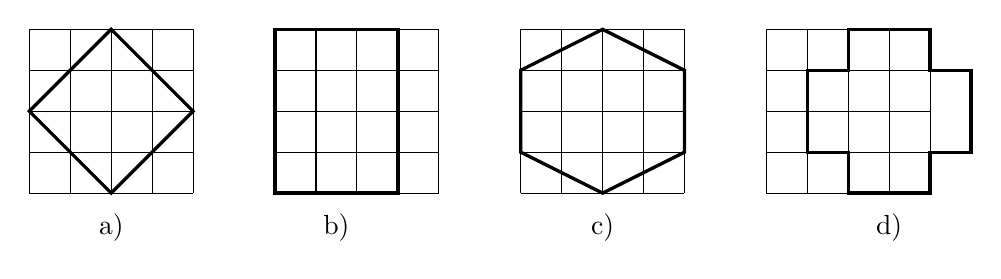
\begin{tikzpicture}[x=0.52cm,y=0.52cm]
                % a)
                \begin{scope}[shift={(0,0)}]
                    \draw[step=1] (0,0) grid (4,4);
                    \draw[very thick] (2,4)--(4,2)--(2,0)--(0,2)--cycle;
                    \node[below=4pt] at (2,0) {a)};
                \end{scope}
                % b)
                \begin{scope}[shift={(6,0)}]
                    \draw[step=1] (0,0) grid (4,4);
                    \draw[very thick] (0,0) rectangle (3,4);
                    \node[below=4pt] at (1.5,0) {b)};
                \end{scope}
                % c)
                \begin{scope}[shift={(12,0)}]
                    \draw[step=1] (0,0) grid (4,4);
                    \draw[very thick] (0,1)--(2,0)--(4,1)--(4,3)--(2,4)--(0,3)--cycle;
                    \node[below=4pt] at (2,0) {c)};
                \end{scope}
                % d)
                \begin{scope}[shift={(18,0)}]
                    \draw[step=1] (0,0) grid (4,4);
                    \draw[very thick] (1,1)--(1,3)--(2,3)--(2,4)--(4,4)--(4,3)--(5,3)--(5,1)--(4,1)--(4,0)--(2,0)--(2,1)--cycle;
                    \node[below=4pt] at (3,0) {d)};
                \end{scope}
            \end{tikzpicture}

            \textit{Hình 9.12}
        \end{center}

        \answerline

        \item Hình nào dưới đây vẽ hai điểm $M$, $N$ thoả mãn phép quay ngược chiều $60^\circ$ tâm $O$ biến $N$ thành $M$?

        \begin{center}
            \begin{tikzpicture}[x=1cm,y=1cm]
                % a
                \begin{scope}[shift={(0,0)}]
                    \coordinate (Oa) at (0,0);
                    \coordinate (Ma) at (2.2,0);
                    \coordinate (Na) at (60:1.75);
                    \draw (Oa)--(Ma) (Oa)--(Na);
                    \draw (0.45,0) arc[start angle=0,end angle=60,radius=.45];
                    \draw (1.05,-.08)--(1.05,.08);
                    \draw ($(Oa)!0.55!(Na)+(-.09,.04)$)--($(Oa)!0.55!(Na)+(.09,-.04)$);
                    \draw ($(Oa)!0.55!(Na)+(-.06,.12)$)--($(Oa)!0.55!(Na)+(.12,.02)$);
                    \node[below left] at (Oa) {$O$};
                    \node[right] at (Ma) {$M$};
                    \node[above] at (Na) {$N$};
                    \node at (.55,.31) {$60^\circ$};
                    \node[below=7pt] at (1.05,0) {a)};
                \end{scope}
                % b
                \begin{scope}[shift={(4.2,0)}]
                    \coordinate (Ob) at (0,0);
                    \coordinate (Mb) at (2.1,0.25);
                    \coordinate (Nb) at (60:2.1);
                    \draw (Ob)--(Mb) (Ob)--(Nb);
                    \draw (0.45,.05) arc[start angle=6.8,end angle=60,radius=.45];
                    \draw ($(Ob)!0.55!(Mb)+(-.02,-.09)$)--($(Ob)!0.55!(Mb)+(.02,.09)$);
                    \draw ($(Ob)!0.55!(Nb)+(-.08,.04)$)--($(Ob)!0.55!(Nb)+(.08,-.04)$);
                    \node[below left] at (Ob) {$O$};
                    \node[right] at (Mb) {$M$};
                    \node[above] at (Nb) {$N$};
                    \node at (.62,.38) {$60^\circ$};
                    \node[below=7pt] at (1.05,0) {b)};
                \end{scope}
                % c
                \begin{scope}[shift={(8.6,0)}]
                    \coordinate (Oc) at (0,0);
                    \coordinate (Nc) at (20:2.1);
                    \coordinate (Mc) at (70:2.1);
                    \draw (Oc)--(Nc) (Oc)--(Mc);
                    \draw (20:.48) arc[start angle=20,end angle=70,radius=.48];
                    \draw ($(Oc)!0.55!(Nc)+(-.03,-.09)$)--($(Oc)!0.55!(Nc)+(.03,.09)$);
                    \draw ($(Oc)!0.55!(Mc)+(-.08,.03)$)--($(Oc)!0.55!(Mc)+(.08,-.03)$);
                    \node[below left] at (Oc) {$O$};
                    \node[right] at (Nc) {$N$};
                    \node[above] at (Mc) {$M$};
                    \node at (.6,.45) {$50^\circ$};
                    \node[below=7pt] at (1.05,0) {c)};
                \end{scope}
                % d
                \begin{scope}[shift={(13,0)}]
                    \coordinate (Od) at (0,0);
                    \coordinate (Nd) at (2.1,0);
                    \coordinate (Md) at (60:2.1);
                    \draw (Od)--(Nd) (Od)--(Md);
                    \draw (0.45,0) arc[start angle=0,end angle=60,radius=.45];
                    \draw ($(Od)!0.55!(Nd)+(-.02,-.09)$)--($(Od)!0.55!(Nd)+(.02,.09)$);
                    \draw ($(Od)!0.55!(Md)+(-.08,.04)$)--($(Od)!0.55!(Md)+(.08,-.04)$);
                    \node[below left] at (Od) {$O$};
                    \node[right] at (Nd) {$N$};
                    \node[above] at (Md) {$M$};
                    \node at (.55,.31) {$60^\circ$};
                    \node[below=7pt] at (1.05,0) {d)};
                \end{scope}
            \end{tikzpicture}

            \textit{Hình 9.13}
        \end{center}

        \answerline

        \item Cho lục giác đều $ABCDEF$ nội tiếp một đường tròn $(O)$. Chứng minh rằng điểm $O$ cách đều tất cả các cạnh của lục giác đều.

        \answerline
        \answerline
        \answerline

        \item Cho một bát giác đều (đa giác đều có 8 cạnh) nội tiếp một đường tròn tâm $O$. Kẻ các đoạn thẳng nối $O$ với các đỉnh của đa giác và chia đa giác thành 8 tam giác nhỏ cân tại đỉnh $O$. Ba góc của mỗi tam giác nhỏ có số đo bằng bao nhiêu?

        \answerline
        \answerline

        \item Cho $A'$, $B'$, $C'$, $D'$, $E'$, $F'$ là trung điểm các cạnh $AB$, $BC$, $CD$, $DE$, $EF$, $FA$ của lục giác đều $ABCDEF$. Chứng minh rằng $A'B'C'D'E'F'$ là một lục giác đều.

        \answerline
        \answerline
        \answerline

        \item Cho tam giác đều $ABC$ nội tiếp đường tròn $(O)$ như Hình 9.14. Hãy cho biết các phép quay thuận chiều lần lượt $120^\circ$; $240^\circ$; $360^\circ$ với tâm $O$ biến các đỉnh $A$, $B$, $C$ thành những điểm nào.

        \begin{center}
            \begin{tikzpicture}[scale=0.8]
                \coordinate (O) at (0,0);
                \coordinate (A) at (90:2);
                \coordinate (B) at (210:2);
                \coordinate (C) at (330:2);
                \draw (O) circle (2);
                \draw (A)--(B)--(C)--cycle;
                \draw (O)--(A) (O)--(B) (O)--(C);
                \draw (135:.55) arc[start angle=135,end angle=255,radius=.55];
                \fill (O) circle (1.2pt);
                \node[above=1pt of A] {$A$};
                \node[left=1pt of B] {$B$};
                \node[right=1pt of C] {$C$};
                \node[below=1pt of O] {$O$};
                \node[left=2pt] at (-.32,.28) {$120^\circ$};
            \end{tikzpicture}

            \textit{Hình 9.14}
        \end{center}

        \answerline
        \answerline

        \item Cho hình vuông $ABCD$ nội tiếp đường tròn $(O)$ như Hình 9.15. Hãy cho biết các phép quay ngược chiều lần lượt $90^\circ$; $180^\circ$; $270^\circ$; $360^\circ$ với tâm $O$ biến các đỉnh $A$, $B$, $C$, $D$ thành những điểm nào.

        \begin{center}
            \begin{tikzpicture}[scale=0.8]
                \coordinate (O) at (0,0);
                \coordinate (A) at (135:2);
                \coordinate (B) at (45:2);
                \coordinate (C) at (-45:2);
                \coordinate (D) at (-135:2);
                \draw (O) circle (2);
                \draw (A)--(B)--(C)--(D)--cycle;
                \fill (O) circle (1.2pt);
                \node[below=1pt of O] {$O$};
                \node[left=1pt of A] {$A$};
                \node[right=1pt of B] {$B$};
                \node[right=1pt of C] {$C$};
                \node[left=1pt of D] {$D$};
            \end{tikzpicture}

            \textit{Hình 9.15}
        \end{center}

        \answerline
        \answerline

        \item Cho lục giác đều $ABCDEF$ nội tiếp đường tròn tâm $O$.
        \begin{questions}
            \item Chứng tỏ $ACE$ là tam giác đều.

            \answerline
            \answerline
            \item Liệt kê ba phép quay giữ nguyên tam giác đều $ACE$.

            \answerline
            \item Liệt kê sáu phép quay giữ nguyên lục giác đều $ABCDEF$.

            \answerline
        \end{questions}

        \item Một phép quay thuận chiều $120^\circ$ tâm $O$ biến điểm $A$ thành điểm $B$, biến điểm $B$ thành điểm $C$. Chứng tỏ rằng $ABC$ là tam giác đều nội tiếp một đường tròn tâm $O$.

        \answerline
        \answerline
        \answerline

        \item Cho $O$ là trung điểm của đoạn thẳng $AB$.
        \begin{questions}
            \item Tìm một phép quay biến điểm $A$ thành điểm $B$ và biến điểm $B$ thành điểm $A$.

            \answerline
            \item Phép quay thuận chiều $90^\circ$ tâm $O$ biến $A$ thành $C$ và biến $B$ thành $D$. Chứng tỏ rằng $ACBD$ là một hình vuông.

            \answerline
            \answerline
            \answerline
        \end{questions}
    \end{questions}
\end{practice}
